\documentclass[conference]{IEEEtran}
\IEEEoverridecommandlockouts

\usepackage{amsmath,amssymb}
\usepackage{graphicx}
\usepackage{booktabs}
\usepackage{multirow}
\usepackage{cite}
\usepackage{url}
\usepackage{microtype}
\usepackage{array}
\usepackage{tikz}
\usetikzlibrary{arrows.meta,positioning,shapes.geometric,fit}
\usepackage{balance}
\usepackage[hidelinks]{hyperref}

\title{Relation-Aware GNN--BERT Fusion for Music Context Understanding}

\author{\IEEEauthorblockN{Anisha Hasnat}
\IEEEauthorblockA{Student ID.: 22301775\\ 
Department of Computer Science and Engineering\\
Project on Neural Networks (CSE425 / EEE474 / CSE715)\\
\texttt{dummy github link}}}

\begin{document}
\maketitle

\begin{abstract}
For music-context understanding, such models are needed which represent both local acoustic evidence and relationship between non-adjacent music segments. This paper investigates multimodal GNN-BERT pipeline on a reproducible subset of the real MagnaTagATune dataset consisting of 500 tracks. It's primary architectural contribution is the \emph{relation-aware temporal/recurrence GraphSAGE} encoder that distinguishes between sequential-adjacency edges and non-local recurrence edges and fuses their messages via a learned element-wise gate before they are fused to the graph--text interaction. To avoid direct leakage of the target text into the model, the 25 prediction labels and 49 lexical variants are not added to the input text for DistilBERT, which instead gets genuine positive non-target MagnaTagATune annotations and catalogue metadata. The relation-aware encoder achieves slightly higher mean Macro-F1 (0.1932 vs. 0.1920) and Micro-F1 (0.2119 vs. 0.2068) scores, while providing lower AUC-PR (0.2657 vs. 0.2735) scores in a controlled three-seed comparison, presenting a trade-off but not a global advantage. The F1 scores are the same for cross-attention and early concatenation in Task~3, but cross-attention performing better on AUC-PR with 0.145 compared to 0.137 for early concatenation. These findings are in line with the feasibility of explicitly modelling temporal continuity and musical recurrence as different graph relations and indicate that the advantage is only small with this small real-data subset.
\end{abstract}

\begin{IEEEkeywords}
music information retrieval, GraphSAGE, graph neural networks, BERT, multimodal fusion, music auto-tagging, MagnaTagATune
\end{IEEEkeywords}

\section{Introduction}
Automatic music tagging is a multi-label prediction problem that allows a music track to have several genre, instrumentation, vocal, tempo and mood related properties. However, as local time--frequency patterns contain a lot of information about timbre and instrumentation \cite{choi2016,pons2019}, spectrogram CNNs continue to provide strong baselines. However, a 2D spectrogram does not directly represent relationships like: a repeated motif comes back after several segments, or a structurally similar phrase is far from the first time it is presented etc.

Graph neural networks (GNNs) provide an complimentary inductive bias by modelling music segments as nodes in a graph and musical structural relationships as edges. Meanwhile, pre-trained language encoders give context to textual music descriptions or annotations. The official project specification works as a motivation to fuse graph-based audio structure and textual context in a GNN--BERT architecture to make multi-label predictions. The main issue of this work is narrower: \emph{should temporal adjacency be considered the same graph-relation as non-local recurrence?}

\textbf{Contribution and novelty.} Relation-specific message passing has been widely used in general graph learning, such as relational GCNs \cite{schlichtkrull2018}. More recently, multimodal music-tagging research has been done with graphs, text, audio and attention \cite{huang2026}. Thus, the novelty of this work does not lie in the ``GNN + BERT" approach or relation-aware GNNs, in particular. The project contribution is to decompose a music segment graph into (i) chronologically ordered temporal edges and (ii) feature similarity recurrence edges, and then apply (iii) learned gate and (iv) graph-to-BERT-token cross-attention. The literature studied for this project did not show previous studies that have investigated this specific temporal/recurrence gated segment encoder in the same music-context fusion setting. Implementation is tested using a 3-seed controlled ablation and gate/degree diagnostics and not with a first-ever claim.

The study provides three concrete contributions: (1) a real-data MagnaTagATune compliance benchmark with artist-grouped splits; (2) a compact relation-aware GraphSAGE layer which preserves the separate temporal and recurrence messages; and (3) controlled comparisons against a mel-spectrogram CNN, BERT-only, vanilla GraphSAGE, early concatenation, and graph-to-text cross-attention.

\section{Related Work}
\subsection{Music Auto-Tagging}
One of the most popular music tagging benchmarks is the MagnaTagATune music benchmark, introduced by \cite{law2009}. Later, strong spectrogram-based baselines were set on this dataset by deep CNN systems \cite{choi2016}. Additionally, Musicnn demonstrated how well musically motivated convolutional architectures and attention could be used for automatic tagging \cite{pons2019}. These methods inspired us to use the mel-spectrogram CNN baseline in this work, and most of them work on grid-structured representations of audio.

\subsection{Graph Representation Learning}
GraphSage learns the node representations inductively by aggregating neighborhood information \cite{hamilton2017}, while Graph Attention Networks learn weights of neighbors \cite{velickovic2018}. Prior to this project, there are multi-relational graph learning approaches such as R-GCN, which explicitly parameterizes relation types \cite{schlichtkrull2018}. Thus, our relation-aware layer is best thought of as a small instance of a music-specific GNN family. It has two relations that are designed to be interpretable: temporal continuity and non-local recurrence.

\subsection{Text and Multimodal Music Models}
BERT offers contextualised representation of tokens which also generalise well to downstream classification tasks \cite{devlin2019}. Audio--text alignment objectives are inspired by contrastive dual encoders like CLIP \cite{radford2021} or InfoNCE-based representation learning \cite{oord2018}, and MusicCaps is a model that generates natural language descriptions of music clips \cite{agostinelli2023}. MuCoGraph is a recent multimodal music-tagging system that brings together four data modalities: audio, BERT-based text, heterogeneous graph and co-attention. The present project has a more focused scope than this more general system: it aims to separate out whether two structural relations between different parts of a single audio segment graph should be aggregated separately prior to BERT fusion.

\section{Dataset and Experimental Protocol}
\subsection{Real MagnaTagATune Subset}
The main criterion includes 500 authentic MagnaTagATune clips. The complete dataset includes approximately 25.9k clips of 29 seconds' duration and 188 binary tags produced manually (Human-generated) \cite{law2009}. There are 18 artists and 25 target labels for the project subset:
\emph{guitar, slow, classical, ambient, female, vocal, techno, electronic, indian, fast, piano, drums, singing, loud, quiet, pop, male vocal, strings, flute, soft, woman, vocals, man, female vocal, female vocals}.

The subset is not meant to be a substitute for the MagnaTagATune benchmarking using the full dataset. It is designed to offer a real data compliance experiment for the project deadline and CPU limits.

\subsection{Artist-Grouped Split}
The final partition contains 342 training tracks (68.4\%), 80 validation tracks (16.0\%), and 78 held-out test tracks (15.6\%). There are 3 validation, 3 test and 12 training artists. The partition was selected to keep the label coverage intact with strict separation of artists. Split constructions took into account the support of the label and therefore the resulting split should be regarded as a project-specific split and not as a canonical public split.

\subsection{Audio Features and Segment Graphs}
The audio is resampled to 22,050~Hz and processed using \texttt{librosa} \cite{mcfee2015}. The tracks are divided in 5 second segments. A 32-dimensional node feature is composed of 12 statistics of the chroma and 12 summary values of the mel bands along with 8 statistics of the MFCC. Two sets of edges are formed:
\begin{itemize}
    \item \textbf{Temporal edges} are the ones that link chronologically adjacent segments.
    \item \textbf{Recurrence edges} are created between non-adjacent segments, whose maximal cosine similarity is at least $\tau=0.65$ and only the 3 nearest recurrence neighbors are kept.
\end{itemize}
There are 3,000 segment nodes in the graph cache of 500 tracks. The mean temporal degree is 1.6667 and the mean recurrence degree is 1.7560, 20.83\% of nodes don't have a recurrence neighbor.

\subsection{Text Input and Leakage Control}
DistilBERT gets real positive MagnaTagATune annotations, \emph{not} included in prediction targets, followed by title, artist and album metadata. Direct lexical leakage is controlled by \emph{not} including all 25 target labels and 49 manually-specified lexical variants from BERT input. No target phrase was excluded from the constructed text by a regex audit. This is a direct lexical leakage check, semantically correlated non-target tags are discussed as a limitation of validity and can provide proxy information.

\subsection{Training and Evaluation}
AdamW is used throughout with batch size of 16 and fixed seed resets. The training for task~1 BERT is done for 20 epochs with cosine decay. For Task~2 GNN models, we use 15 epochs and we repeat vanilla and relation-aware GraphSAGE for seeds 42, 43 and 44 in the controlled novelty experiment. Task~3 is a two-phase schedule, with 10 epochs of pretrained encoders being frozen, and 5 epochs of the top two DistilBERT blocks being unfrozen and trained with a smaller learning rate.

The implementation for F1 evaluation uses a fixed probability threshold of 0.30, if no probability is above threshold, the two top probabilities labels are selected. These decisions are then used to calculate Macro-F1 and Micro-F1. AUC-PR is macro-averaged for the subset of labels that have positive test support, that is, at least one positive test example in the 25 retained labels. This decision rule is retained for all the compared models.

\section{Problem Formulation and Baselines}
Each music clip is represented by
\begin{equation}
T=(X_a,X_t,G,y),
\end{equation}
where $X_a$ contains acoustic features, $X_t$ is non-leaking textual context, $G=(V,E_t\cup E_r)$ is the segment graph, and $y\in\{0,1\}^{25}$ is the multi-label target vector. For each label $k$, models output $\hat y_k=\sigma(o_k)$. Training minimizes weighted binary cross-entropy
\begin{equation}
\mathcal{L}_{tag}=-\frac{1}{K}\sum_{k=1}^{K}\left[w_k y_k\log \hat y_k+(1-y_k)\log(1-\hat y_k)\right],
\end{equation}
with a fixed positive-class weight of 3.5 in the real-data runs.

The comparison is not very extensive. It was an intentional approach. B1 is a majority/random-prior predictor based on the frequencies of the training labels. B2 is a 3-layer 2D CNN, which is operating on log-mel spectrograms. Task~1 only requires DistilBERT. Task~2 is a comparison between vanilla and relation-aware GraphSAGE on identical segment graphs. Task~3 is the same as Task~2 with the addition of a cross-attention model between the graph and the tokens, and with a fixed relation-aware audio backbone. There is also a contrastive dual-encoder model for Task~4 in the repository, but the results it returns with synthetic pipelines are not used as evidence in the primary real-data benchmark.

For evaluation, per-label precision and recall are
\begin{equation}
P_k=\frac{TP_k}{TP_k+FP_k},\qquad R_k=\frac{TP_k}{TP_k+FN_k},
\end{equation}
and $F1_k=2P_kR_k/(P_k+R_k)$. 

Macro-F1: averages $F1_k$ over the labels. 

Micro-F1: pools decisions across all the labels and then compute F1. 

AUC-PR is calculated from probabilities, and it is highlighted because the distribution of the labels is imbalanced.

\section{Proposed Relation-Aware GNN--BERT Model}
\subsection{Vanilla GraphSAGE Baseline}
Given node states $h_i^{(l)}$, vanilla GraphSAGE aggregates all neighbors in a single pool:
\begin{equation}
\bar{m}_i^{(l)} = \frac{\sum_{j\in \mathcal{N}(i)} w_{ji} h_j^{(l)}}{\sum_{j\in \mathcal{N}(i)} w_{ji}+\epsilon},
\end{equation}
\begin{equation}
h_i^{(l+1)} = W_s h_i^{(l)} + W_n \bar{m}_i^{(l)} + b.
\end{equation}
The neighborhood statistic is thus the same for both temporal and recurrence edges.

\subsection{Relation-Aware Aggregation}
The proposed layer uses separate weighted means:
\begin{align}
m_{i,t}^{(l)} &= \frac{\sum_{j\in\mathcal{N}_{t}(i)}w_{ji}h_j^{(l)}}{\sum_{j\in\mathcal{N}_{t}(i)}w_{ji}+\epsilon},\\
m_{i,r}^{(l)} &= \frac{\sum_{j\in\mathcal{N}_{r}(i)}w_{ji}h_j^{(l)}}{\sum_{j\in\mathcal{N}_{r}(i)}w_{ji}+\epsilon}.
\end{align}
A vector-valued gate is then learned element-wise:
\begin{equation}
\gamma_i = \sigma\!\left(W_g[h_i^{(l)}\Vert m_{i,t}^{(l)}\Vert m_{i,r}^{(l)}]\right),
\end{equation}
\begin{equation}
m_i^{(l)} = \gamma_i\odot m_{i,t}^{(l)}+(1-\gamma_i)\odot m_{i,r}^{(l)}.
\end{equation}
The node update is
\begin{equation}
h_i^{(l+1)}=W_s h_i^{(l)}+W_n m_i^{(l)}+b.
\end{equation}
When there are only temporal neighbours, it is required that $\gamma_i=1$; when there are only recurrence neighbours, it is required that $\gamma_i=0$. The track representation is a global mean pooling which yields $g\in\mathbb{R}^{64}$. The mean for the audit on this learned gate is 0.5285, and the standard deviation is 0.2183, meaning that there is no complete average collapse to one relation.

\subsection{BERT Fusion}
The BERT baseline is based on the usage of the contextual text representation $H_{text}$ and its pooled vector $t$. Early fusion concatenates $[g\Vert t]$. Cross-attention, on the other hand, applies the graph vector as query to the token embeddings:
\begin{align}
Q &= gW_Q,\quad K=H_{text}W_K,\quad V=H_{text}W_V,\\
A &= \operatorname{softmax}\left(\frac{QK^\top}{\sqrt{d_k}}\right),\\
z &= [g\Vert AV].
\end{align}
A multi-label head predicts 25 sigmoid probabilities for $z$.

\begin{figure*}[t]
\centering
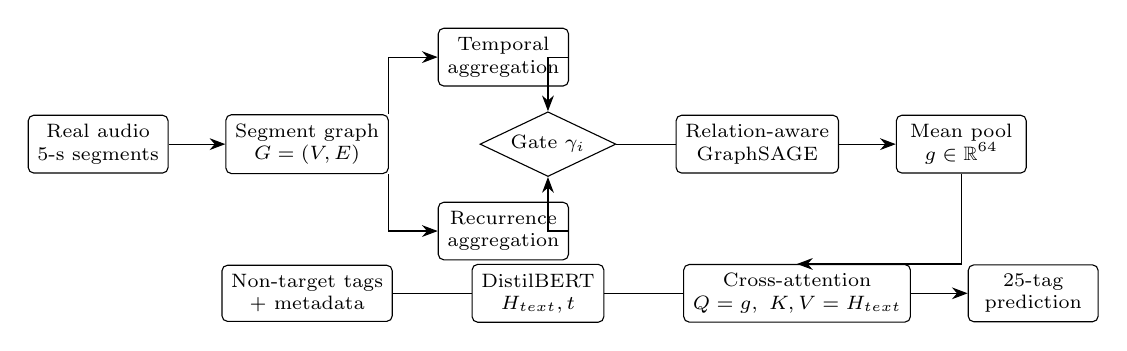
\begin{tikzpicture}[
  node distance=0.55cm and 0.72cm,
  blk/.style={rectangle,draw,rounded corners=2pt,minimum height=0.55cm,minimum width=1.65cm,align=center,font=\scriptsize},
  sml/.style={rectangle,draw,rounded corners=2pt,minimum height=0.48cm,minimum width=1.45cm,align=center,font=\scriptsize},
  gate/.style={diamond,draw,aspect=2.1,align=center,font=\scriptsize,inner sep=1.5pt},
  arr/.style={-{Stealth[length=2mm]},thin}
]
\node[blk] (audio) {Real audio\\5-s segments};
\node[blk,right=of audio] (graph) {Segment graph\\$G=(V,E)$};
\node[sml,above right=0.35cm and 0.62cm of graph] (temp) {Temporal\\aggregation};
\node[sml,below right=0.35cm and 0.62cm of graph] (rec) {Recurrence\\aggregation};
\node[gate,right=1.15cm of graph] (g) {Gate $\gamma_i$};
\node[blk,right=0.75cm of g] (sage) {Relation-aware\\GraphSAGE};
\node[blk,right=of sage] (pool) {Mean pool\\$g\in\mathbb{R}^{64}$};
\node[blk,below=1.15cm of graph] (text) {Non-target tags\\+ metadata};
\node[blk,right=1.0cm of text] (bert) {DistilBERT\\$H_{text},t$};
\node[blk,right=1.0cm of bert] (attn) {Cross-attention\\$Q=g,\ K,V=H_{text}$};
\node[blk,right=of attn] (head) {25-tag\\prediction};
\draw[arr] (audio)--(graph);
\draw[arr] (graph.north east)|-(temp.west);
\draw[arr] (graph.south east)|-(rec.west);
\draw[arr] (temp.east)-|(g.north);
\draw[arr] (rec.east)-|(g.south);
\draw[arr] (g)--(sage)--(pool);
\draw[arr] (text)--(bert)--(attn)--(head);
\draw[arr] (pool.south)|-(attn.north);
\end{tikzpicture}
\caption{Proposed pipeline. The audio graph maintains temporal and recurrence relationships until a learned gate merges their messages. The representations of the BERT tokens are then queried by the pooled graph embedding using cross attention.}

\label{fig:architecture}
\end{figure*}

\section{Results}
\begin{table}[t]
\caption{Primary Real-Data Benchmark (Seed 42)}
\label{tab:primary}
\centering
\footnotesize
\setlength{\tabcolsep}{3.2pt}
\begin{tabular}{lccc}
\toprule
Model & Macro-F1 & Micro-F1 & AUC-PR\\
\midrule
Random/Majority & 0.006 & 0.035 & 0.097\\
Mel-spectrogram CNN & \textbf{0.200} & \textbf{0.223} & 0.250\\
BERT-only & 0.055 & 0.116 & 0.126\\
Vanilla GraphSAGE & 0.199 & 0.213 & 0.277\\
Relation-aware GraphSAGE & 0.190 & 0.213 & \textbf{0.279}\\
Early concatenation & 0.169 & 0.177 & 0.137\\
Cross-attention & 0.169 & 0.177 & 0.145\\
\bottomrule
\end{tabular}
\end{table}

\begin{figure}[t]
\centering
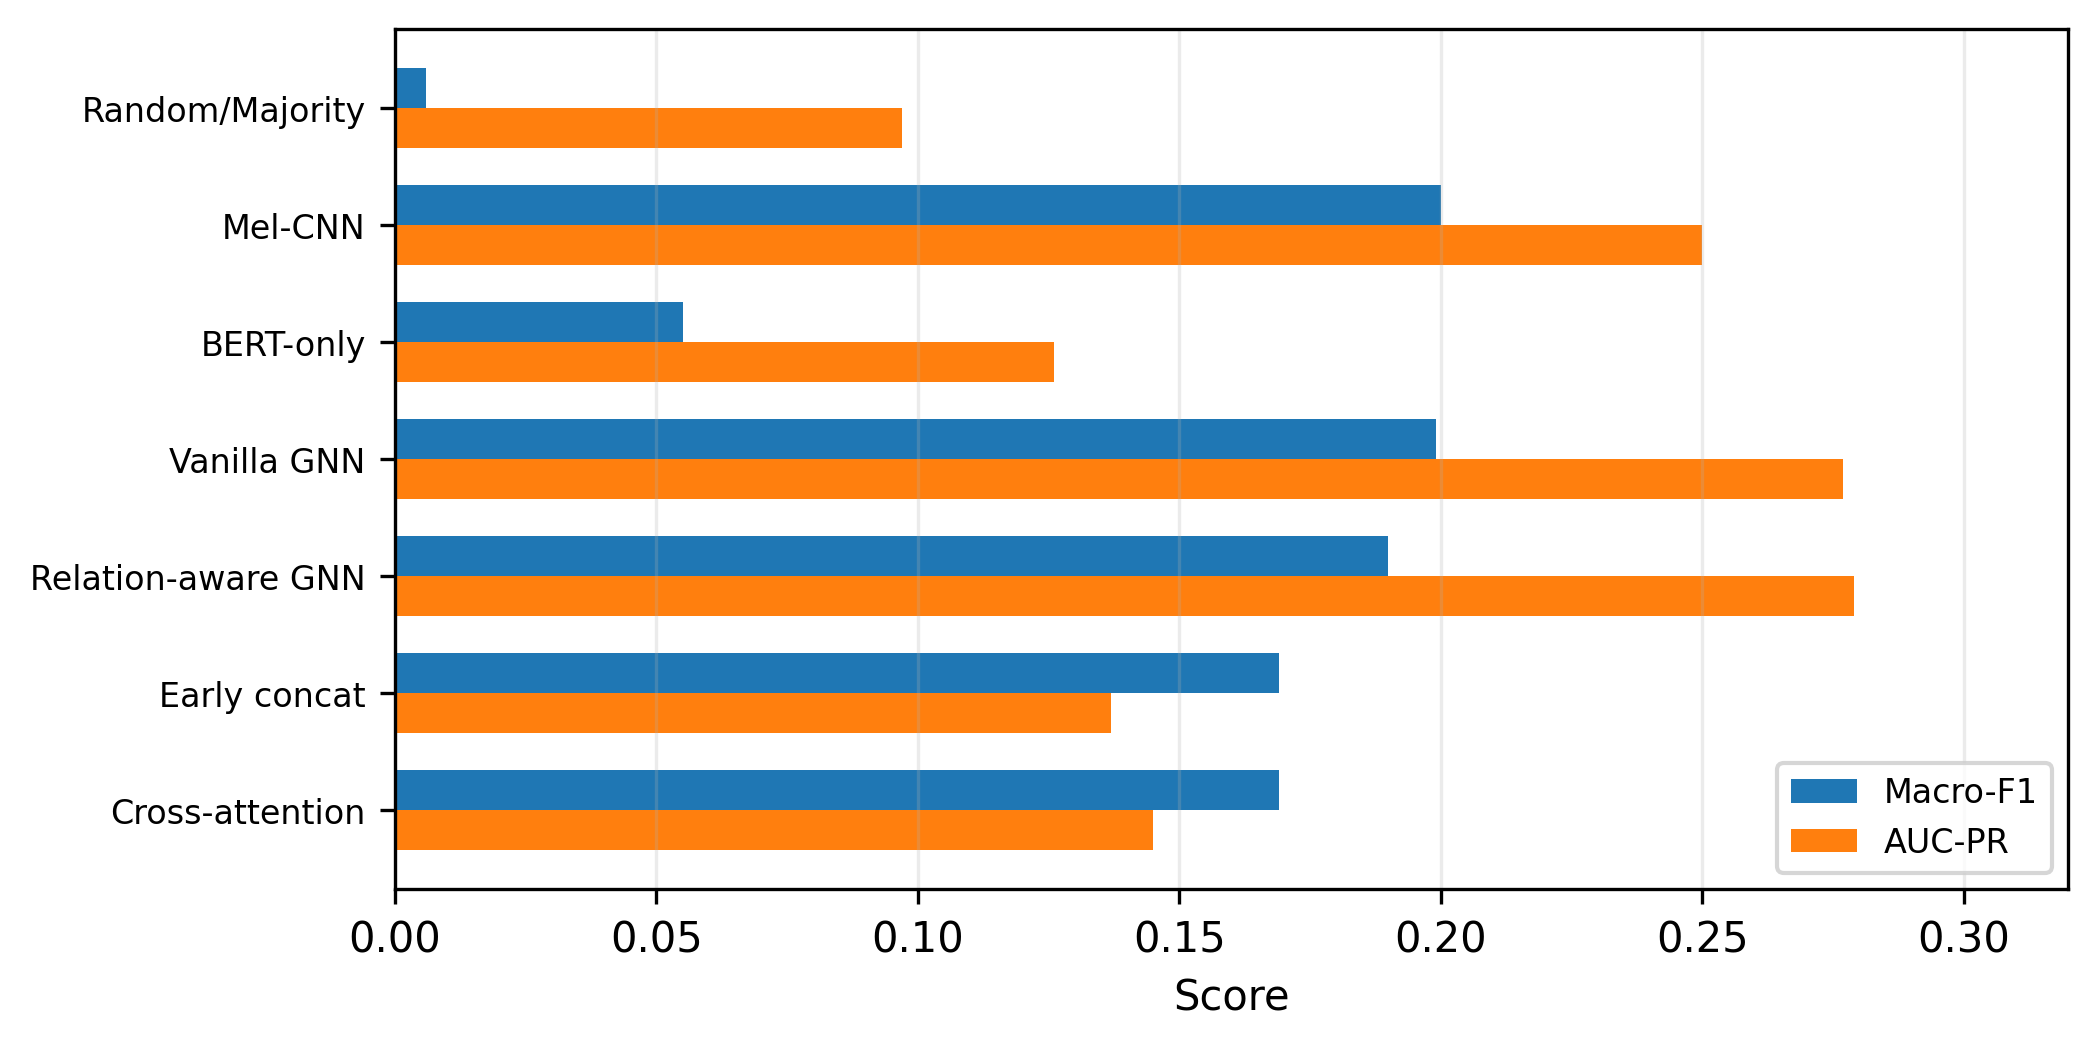
\includegraphics[width=\columnwidth]{real_benchmark_compact.png}
\caption{Seed-42 Macro-F1 and AUC-PR on the 500-track real-data benchmark. No single model dominates all metrics.}
\label{fig:benchmark}
\end{figure}

As seen from Table~\ref{tab:primary}, the mel-spectrogram CNN achieves the highest seed-42 Macro-F1 and Micro-F1 while the relation-aware GraphSAGE achieves the highest AUC-PR. The audio-only GNNs significantly outperform BERT-only GNNs, which means that non-target textual context is weak in the artist-disjoint evaluation scenario. Notably, the proposed relation-aware encoder does not outperform vanilla GraphSAGE uniformly as it shows lower Macro-F1 (0.190 vs. 0.199), but tied Micro-F1 after rounding and slightly higher AUC-PR (0.279 vs. 0.277) over the single-seed table.

\subsection{Three-Seed Novelty Ablation}
\begin{table}[t]
\caption{Controlled Three-Seed GNN Ablation (Mean $\pm$ Std.)}
\label{tab:multiseed}
\centering
\scriptsize
\setlength{\tabcolsep}{2.8pt}
\begin{tabular}{lccc}
\toprule
Encoder & Macro-F1 & Micro-F1 & AUC-PR\\
\midrule
Vanilla & $0.1920\pm0.0070$ & $0.2068\pm0.0051$ & $\mathbf{0.2735\pm0.0029}$\\
Relation-aware & $\mathbf{0.1932\pm0.0040}$ & $\mathbf{0.2119\pm0.0036}$ & $0.2657\pm0.0098$\\
\bottomrule
\end{tabular}
\end{table}

\begin{figure}[t]
\centering
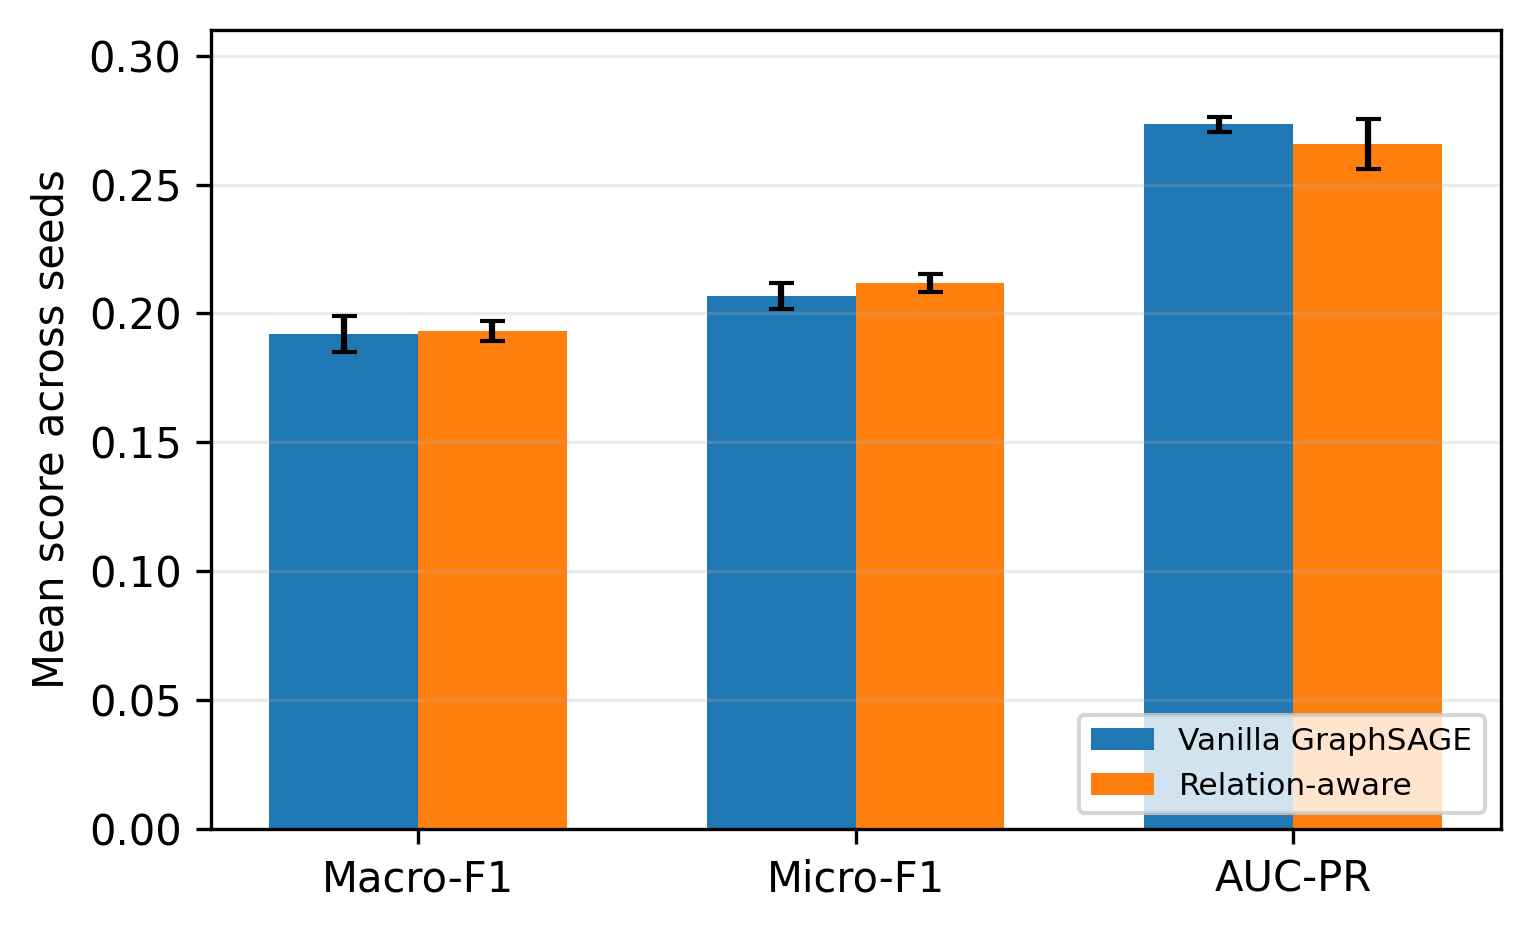
\includegraphics[width=0.95\columnwidth]{multiseed_ablation.png}
\caption{Mean $\pm$ standard deviation over seeds 42, 43, and 44. Relation-aware GraphSAGE slightly raises mean F1 but lowers mean AUC-PR.}
\label{fig:multiseed}
\end{figure}

Overall, across seeds, the relation-aware encoder improves the mean Macro-F1 by 0.0012 and the mean Micro-F1 by 0.0051, and decreases AUC-PR by 0.0078. The improvement is \emph{not} uniform on a seed-wise basis: Macro-F1 is lower at seed 42 and 43, and higher at seed 44. So the evidence points toward feasibility of the architecture, and a small average benefit for F1, but not to a remarkable advantage of the architecture. The relation-aware model also shows higher AUC-PR standard deviation, indicating higher sensitivity of the ranking to the initialisation.

\subsection{Fusion Ablation}
The Macro-F1 scores for early concatenation and cross-attention are 0.169 and 0.177, respectively. The Cross-attention improves AUC-PR by 0.008 (from 0.137 to 0.145). This only means that there is a slight improvement at the fixed decision threshold and there is a slight improvement in the probability ranking. Since both fusion variants are still below the level of the audio-only GNNs, no improvement of the primary classification metrics on this subset is obtained by adding the available text.

\begin{figure}[t]
\centering
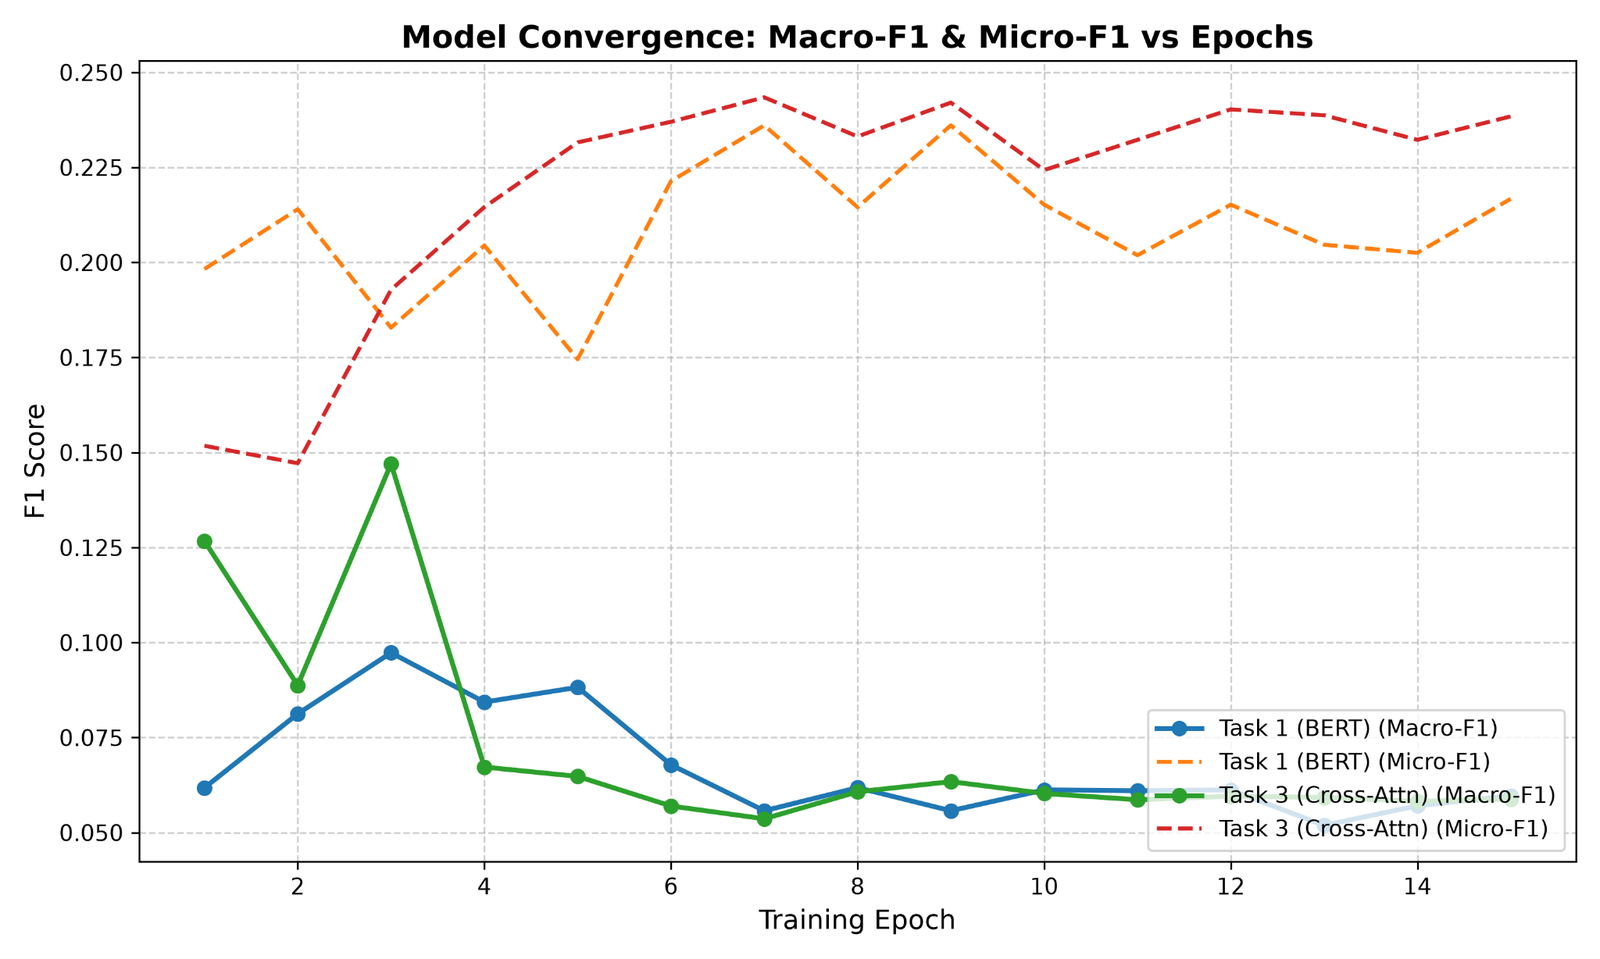
\includegraphics[width=\columnwidth]{mtt_f1_curves_resized.png}
\caption{From the real MagnaTagATune correction run, Validation F1 trajectories. The final test table is using the chosen saved checkpoints and so does not have to be the same as the last plotted validation epoch.}
\label{fig:convergence}
\end{figure}


\subsection{Per-Seed Behavior}
The mixed nature of the novelty result is explicitly evident from Table~\ref{tab:perseed}. As the paper indicates, Relation-aware GraphSAGE is not better at every seed and at every metric, and hence taking the mean $\pm$ standard deviation of the runs instead of a favourable one.

\begin{table}[t]
\caption{Per-Seed Vanilla vs. Relation-Aware GNN Results}
\label{tab:perseed}
\centering
\scriptsize
\setlength{\tabcolsep}{2.5pt}
\begin{tabular}{c l c c c}
\toprule
Seed & Encoder & Macro-F1 & Micro-F1 & AUC-PR\\
\midrule
42 & Vanilla & 0.1986 & 0.2135 & 0.2772\\
42 & Relation-aware & 0.1897 & 0.2128 & 0.2788\\
43 & Vanilla & 0.1952 & 0.2058 & 0.2733\\
43 & Relation-aware & 0.1912 & 0.2158 & 0.2629\\
44 & Vanilla & 0.1824 & 0.2011 & 0.2701\\
44 & Relation-aware & 0.1987 & 0.2071 & 0.2553\\
\bottomrule
\end{tabular}
\end{table}

The seed-42 relation-aware model achieves a slightly higher AUC-PR than the others, at the expense of being slightly lower on F1; seed~43 increases Micro-F1, but not Macro-F1 or AUC-PR, and seed~44 increases the scores for both F1 measures while decreasing AUC-PR. The conservative interpretation is supported by this pattern: When model behavior is changed by separating relation types, it changes measurably, but the 500-track benchmark is too small to make any strong claims of superiority.


\section{Class Support and Diagnostic Evidence}
The split is totally artist-disjoint, but is also small. The total number of test clips is 78 and the counts of the labels are positive, as shown in Table~\ref{tab:support}. The most common test label is \emph{indian} with 22 positive cases, while five test labels have only two positives. This imbalance is a part of the reason for the sometimes contradictory nature of AUC-PR and thresholded F1 and why claims of per-class superiority are avoided in the paper.

\begin{table}[t]
\caption{Positive Label Support in the 78-Clip Test Split}
\label{tab:support}
\centering
\scriptsize
\setlength{\tabcolsep}{3pt}
\begin{tabular}{l r l r}
\toprule
Tag & Pos. & Tag & Pos.\\
\midrule
indian & 22 & techno & 18\\
vocal & 17 & woman & 15\\
female & 14 & fast & 11\\
vocals & 10 & loud & 10\\
electronic & 8 & female vocals & 8\\
drums & 7 & slow & 6\\
singing & 5 & quiet & 5\\
guitar & 4 & ambient & 4\\
pop & 4 & female vocal & 4\\
flute & 4 & soft & 3\\
classical & 2 & piano & 2\\
strings & 2 & male vocal & 2\\
man & 2 & & \\
\bottomrule
\end{tabular}
\end{table}

Additionally, there are close related lexical labels used as a target vocabulary like: \emph{vocal}/\emph{vocals} and \emph{female vocal}/\emph{female vocals}. This is in fact the original annotation vocabulary and not a consciously de-duplicated ontology. Thus, Macro-F1 is not a taxonomy-normalized measure of the quality of semantic tagging, but rather a measure of performance on the project label set selected.

The learned gate is another diagnostic. The averaged (over nodes and over feature dimensions) mean of 0.5285 and standard deviation of 0.2183 indicates that not every message was trivially routed through only the temporal or through only the recurrence stream. That does not necessarily mean that both of the relationships are always useful, but it's an indication that the mechanism is working and that the mixed predictive results are not due to an obvious gate-collapse failure.

\section{Discussion}
\subsection{What the Experiment Supports}
Best "conclusion" is not cutting-edge performance, but structural. The relation-aware layer is working as expected: Temporal and recurrence channels are filled up on average, zero-recurrence nodes are treated correctly and learned gate does not saturate globally, it stays around 0.53. The three-seed study presents a small mean F1 improvement, which is mitigated by the mixed per-seed behavior and the lower AUC-PR and thus does not allow for claiming a general predictive improvement.

The negative finding of the fusion is also useful. As for this benchmark, no additional information from non-target human annotations nor catalogue metadata are sufficient to overcome the audio GNN. Slightly better AUC-PR performance is obtained by performing cross-attention as compared to early concatenation, but both fusion models perform worse than audio-only encoders. This indicates that using more complex paired language such as natural captions for future evaluation of graph-to-token attention might be more suitable.

\subsection{Threats to Validity}
There are four limitations that are important. Firstly, only 500 MagnaTagATune clips and 18 artists are used; results are not directly comparable with scores published for full datasets. Only a few dozen clips are available for each label; per-label metric is potentially unstable due to small number of samples, including only a few positives or negatives, in the held-out set. Second, this split was chosen based on an artist-centric approach but without discarding the support of the test labels; hence it is a project split, not an untouched canonical split. Third, there are a number of target labels that are lexically or semantically related to each other (e.g., \emph{vocal}/\emph{vocals}/\emph{female vocal}/\emph{female vocals}), and removing direct lexical variants does not remove all the semantic proxy information from the BERT input. Fourth, the threshold value of 0.30 (with top-2 fallback) has an impact on the behavior of F1 and should be left unchanged when reproducing the table.

Additionally, PR curve, t-SNE, retrieval and qualitative artifacts from another synthetic pipeline-validation stage are included. Although these artifacts can be used to check the sanity of the code, they are not included in the main real-data claims in this paper. Likewise, the contrastive Task~4 implementation was ad hoc, and the real-data compliance pass was focused on Tasks~1--3, and a retrieval Match MusicCaps type pass was not available.


\section{Project Scope and Compliance}
The taskmap of the final paper is summarized in Table~\ref{tab:taskmap}. The real-data compliance pass focuses on Tasks~1-3 as these tasks can be objectively assessed with MagnaTagATune audio and human tags. Task~4 is still in place as an optional contrastive extension in the repository, but the retrievals which were reported previously were from the synthetic sanity-check pipeline and are not included in the real-data tables.

\begin{table}[t]
\caption{Final Project Task Mapping}
\label{tab:taskmap}
\centering
\scriptsize
\setlength{\tabcolsep}{3pt}
\begin{tabular}{p{0.7cm}p{2.25cm}p{2.7cm}}
\toprule
Task & Model & Evidence in this paper\\
\midrule
1 & DistilBERT tagger & Real MTT Macro/Micro-F1, AUC-PR\\
2 & Vanilla / relation-aware GNN & Real MTT benchmark + 3-seed ablation\\
3 & Early concat / cross-attention & Real MTT fusion comparison\\
4 & Contrastive dual encoder & Code retained; primary metrics not claimed\\
\bottomrule
\end{tabular}
\end{table}

The synthetic 100-track generator remains only as a convenience to facilitate unit testing, quick end-to-end testing, and to exercise optional code paths in the absence of public data. It's obvious that it's clean and easily distinguished from the primary MagnaTagATune artifacts in the repository. This distinction is significant as synthetic labels, captions, or emotion values cannot replace the evaluation of public-datasets.

\subsection{Ethical and Reproducibility Considerations}
The labels MagnaTagATune collect from the human annotation consist of subjective concepts, correlated descriptors and demographic/vocal terms. The model thus learns conventions and biases found in those labels – predictions should not be regarded as objective descriptions of the identity or quality of music. Only catalogue text is used as a model input and is split by the artist to minimize the memorization of the production or identity-specific cues.

To ensure reproducibility, the final report separates measured values from qualitative interpretation, makes the random seeds visible and explicitly saves the split IDs and the metric JSON files. To intentionally report all the outcomes per seed, the 3-seed ablation is reported as well, even if the proposed encoder is worse. This prevents the selection of only the most favourable run and allows the small effect size to be seen by the reader.

\section{Reproducibility}
The codebase is divided into raw data, processed graph caches, split files, model checkpoints, plots and report artifacts. The main real data files are separate from the synthetic sanity-check files. Whereas the relation-aware implementation can handle an explicit edge-type if present in the graph, it can also identifies temporal edges from neighboring segment indices and recurrence edges from the complementary relation. The last three-seed values are in \texttt{magnatagatune\_ablation\_multiseed.json}. The project test suite includes 12 tests that pass in the areas of feature extraction, graph building, encoders, fusion, contrastive code, baselines, and relation-aware layers.

\section{Conclusion}
This project tested a compact relation-aware GNN--BERT architecture on the real-world subset of MagnaTagATune consisting of 500 tracks for music-context tagging. The proposed encoder which distinguish temporal continuity from the non-local recurrence and learns an element-wise gating before GraphSAGE propagation. In three seeds, while relation-aware GraphSAGE outperforms vanilla GraphSAGE in terms of mean Macro-F1 and Micro-F1 scores, it underperforms in terms of AUC-PR; therefore, it can be considered as a meaningful structural design with mixed performance evidence, instead of a universally better model. As can be seen, cross-attention provides a slightly higher AUC-PR score than early concatenation, but not higher F1 scores. Future work will consider evaluating the same relation-aware graph design with larger canonical split and with more complex paired captions, allowing for a more direct evaluation of graph-to-language attention.

\begin{thebibliography}{00}
\bibitem{law2009} E. Law, L. von Ahn, R. Dannenberg, and M. Crawford, ``Evaluation of algorithms using games: The case of music tagging,'' in \emph{Proc. 10th Int. Soc. Music Inf. Retrieval Conf. (ISMIR)}, 2009.
\bibitem{choi2016} K. Choi, G. Fazekas, and M. Sandler, ``Automatic tagging using deep convolutional neural networks,'' in \emph{Proc. 17th Int. Soc. Music Inf. Retrieval Conf. (ISMIR)}, 2016, pp. 805--811.
\bibitem{pons2019} J. Pons and X. Serra, ``musicnn: Pre-trained convolutional neural networks for music audio tagging,'' arXiv:1909.06654, 2019.
\bibitem{hamilton2017} W. L. Hamilton, R. Ying, and J. Leskovec, ``Inductive representation learning on large graphs,'' in \emph{Advances in Neural Information Processing Systems}, vol. 30, 2017.
\bibitem{velickovic2018} P. Veli\v{c}kovi\'c, G. Cucurull, A. Casanova, A. Romero, P. Li\`o, and Y. Bengio, ``Graph attention networks,'' in \emph{Int. Conf. Learning Representations (ICLR)}, 2018.
\bibitem{schlichtkrull2018} M. Schlichtkrull, T. N. Kipf, P. Bloem, R. van den Berg, I. Titov, and M. Welling, ``Modeling relational data with graph convolutional networks,'' in \emph{The Semantic Web -- ESWC 2018}, pp. 593--607, 2018.
\bibitem{devlin2019} J. Devlin, M.-W. Chang, K. Lee, and K. Toutanova, ``BERT: Pre-training of deep bidirectional transformers for language understanding,'' in \emph{Proc. NAACL-HLT}, 2019, pp. 4171--4186.
\bibitem{radford2021} A. Radford \emph{et al.}, ``Learning transferable visual models from natural language supervision,'' in \emph{Proc. Int. Conf. Machine Learning (ICML)}, 2021, pp. 8748--8763.
\bibitem{oord2018} A. van den Oord, Y. Li, and O. Vinyals, ``Representation learning with contrastive predictive coding,'' arXiv:1807.03748, 2018.
\bibitem{agostinelli2023} A. Agostinelli \emph{et al.}, ``MusicCaps: Generating captions for music audio,'' arXiv:2301.11325, 2023.
\bibitem{mcfee2015} B. McFee, C. Raffel, D. Liang, D. P. W. Ellis, M. McVicar, E. Battenberg, and O. Nieto, ``librosa: Audio and music signal analysis in Python,'' in \emph{Proc. 14th Python in Science Conf.}, 2015, pp. 18--25.
\bibitem{defferrard2017} M. Defferrard, K. Benzi, P. Vandergheynst, and X. Bresson, ``FMA: A dataset for music analysis,'' in \emph{Proc. 18th Int. Soc. Music Inf. Retrieval Conf. (ISMIR)}, 2017, pp. 316--323.
\bibitem{huang2026} Y. Huang, D.-R. Liu, and Y.-H. Chen, ``A multimodal graph-based music auto-tagging framework: Integrating social and content intelligence,'' \emph{Information Technology and Management}, 2026, doi: 10.1007/s10799-026-00496-3.
\end{thebibliography}

\end{document}
